\begin{wrapfigure}[]{R}[0pt]{0.68\textwidth}
  % R - floating; r - h! [narrow lines] <- reduce whitespace below [17]
  \centering
  \includegraphics[width=0.66\textwidth]{evolution_of_climate_models}
  \caption{A growth and evolution timeline of climate models. The complexity of global climate models has increased enormously over the last four decades. The most powerful models, such as the \gls{cesm}, now have the capability of simulating a broad range of atmospheric processes, such as the impact of marine ecosystems on the atmosphere. \copyright \gls{ncar}.}
  \label{fig:growth_esm}
\end{wrapfigure}

\glspl{esm} have been rapidly evolving over the past decades (Fig.~\ref{fig:growth_esm}) thanks to growing computing power. But this development comes at the cost of a complexity rivaling the real world and immense resources for computing. To predict the response of the Earth’s ecosystem in a changing climate and its feedback on the very same climate, it is important to replace past parameterizations with our state-of-the-art understanding of the underlying processes. From solving the Navier-Stokes equations of wind and waves several decades ago, ESMs came to represent even biotical process of soil microbial and fungi. But the more we learn the more do we know what is left unknown. There are missing links and knowledge gaps especially when it comes to the details of the complex interaction between terrestrial ecosystems and the atmosphere. First analyses of \gls{cmip}~6 indicate a growing divergence between models, in particular in the land and atmospheric components. Although this will not revoke climate change, it still affects the reliability of model predictions.

\begin{wrapfigure}[]{R}[0pt]{0.5\textwidth}
  % R - floating; r - h! [narrow lines] <- reduce whitespace below [17]
  \centering
  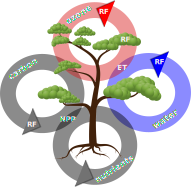
\includegraphics[width=0.48\textwidth]{ozone_es_scheme}
  \caption{Schematic view of the importance of ozone in \glspl{esm}. Ozone inflicts damage to vegetation. Ozone affects photosynthesis negatively and hence \gls{npp} ($\rightarrow$ carbon cycle). Ozone affects opening and closing of stomata (positively and negatively) and hence \gls{et} of plants ($\rightarrow$ water cycle). Both affect the processing of nutrients ($\rightarrow$ nutrient cycle). Ozone damage on vegetation causes positive and negative feedback on tropospheric ozone concentrations and hence on air quality and \gls{rf} \parencite{Nat:Sitch2007}.}
  \label{fig:ozone_esm_scheme}
\end{wrapfigure}

Ozone is an important trace gas in the atmosphere. In accordance with its effects and realm of occurence, we can distinguish the good (stratosphere), the bad (troposphere), and the ugly (ambient air) ozone. Here we shall focus on the connection and feedback between the bad and the ugly sides of ozone. Ozone is ranked third amongst the most potent climate forcers. It contributes to warming in the troposphere where it is produced as a secondary air pollutant in chemical cycles involving precursors such as CO and NOx as well as hydrocarbons (VOC, BVOC). Ozone is highly toxic and harmful to human health and many ecosystems. Despite a successful reduction of precursors in recent years leading to a stagnation of the upward trend in tropospheric ozone concentrations, there are indications that climate feedback on the ozone uptake by land biosphere can hamper reaching the ultimate air quality goal \parencite{NCC:Lin2020}. In drought conditions, plants will limit their transpiration by closing their stomata, which regulate all gas exchange of the plant, while emitting BVOCs at the same time and thus increase surface ozone concentrations. Ozone uptake through plants’ stomata is considered one of the most effective removal pathways of ozone, which will lead to a double penalty of climate change on vegetation and air quality. But large uncertainties in non-stomatal removal remain \parencite{RG:Clifton2020}.
Besides air quality consideration, ozone interferes with the climate and Earth system both directly and indirectly. Directly ozone affects the radiative forcing through its absorbance in both long and short wave bands and hence our assessment on climate change. In this project I will focus on indirect feedback on climate and air quality through ozone impact on vegetation. A high cumulative uptake of ozone (CUO) leads to considerably visible (e.g. necrosis, early senescence) and invisible damage (e.g. reduced photosynthesis) on vegetation (enter citations here). Ozone damage reduces plant photosynthesis and stomatal conductance and therefore interferes directly with net primary production (NPP) and (evapo)transpiration (ET) (Fig.~\ref{fig:schema_ozone_esm}). As depicted in Fig.~\ref{fig:schema_ozone_esm}, ozone uptake by vegetation and consequent damage, interfere with several sensitive parts of the Earth system. Ozone stress affects net primary production (NPP) and gross primary production (GPP) and hence CO2 removal from the atmosphere. Which has consequences on the nutrient cycle. At the same time, physical damage will alter evapotranspiration (ET) of the plant. Depending on the species and severity of damage both a reduced or an increased have been reported \parencite{SR:Hoshika2015}. 
Accounting for ozone induced reduction of stomatal conductance and photosynthesisI independently, \textcite{BGS:Lombardozzi2012} could improve model predictions of GPP and transpiration on global scales. \textcite{BGSD:Franz2020} show potential ozone damage on vegetation under climate change scenarios involving explicit modeling on the plant physiological level. These previous studies have not included an online atmospheric chemistry with known caveats. 
Empirically it was found that ozone damage leads to a reduced maximum electron transport rate $\mathrm{J_{max}}$ and maximum carboxylation efficiency Vcmax \parencite{EJA:Emberson2018} which are the basic processes involved in photosynthesis. Because the ratio $\mathrm{J_{max}}$:Vcmax is found to be constant (even under ozone exposure), the main traits of ozone induced damage can be modeled by a relative reduction in $\mathrm{J_{max}}$ alone (Falk et al., 2021 in preparation)\parencites{BGS:Franz2017}{BGS:Franz2018}.
Here, we want to combine the efforts of process understanding at the vegetation level into a fully coupled ESM with atmospheric chemistry and state-of-the-art nutrient limited carbon sequestration and study the feedback of ozone damage and thermal stress on air quality targets and climate.



